\documentclass[10pt, xcolor=dvipsnames]{beamer}
%\documentclass[10pt, xcolor=dvipsnames,notes=only]{beamer}
%\mode<presentation>
%{
\usetheme{Goettingen}
%\setbeamercovered{transparent}
%} 
\usefonttheme{professionalfonts}
%\usecolortheme{beaver}

\usepackage{setspace}
\usepackage[english]{babel}
\usepackage[latin1]{inputenc}
\usepackage{times}
\usepackage[T1]{fontenc}
\usepackage{color}
\usepackage{graphicx}
\usepackage{amssymb}
\usepackage{amsthm}
\usepackage{bm}
\usepackage{rotating}
\usepackage{ccaption}
\usepackage{booktabs}
\usepackage{lscape}
\usepackage{colortbl}
\usepackage{arydshln}
\usepackage{tabularx}
\usepackage{graphics}
\usepackage{epstopdf}

\setbeamertemplate{navigation symbols}{}
\setbeamertemplate{items}[balls]

\newenvironment{changemargin}[2]{%
  \begin{list}{}{%
    \setlength{\topsep}{0pt}%
    \setlength{\leftmargin}{#1}%
    \setlength{\rightmargin}{#2}%
    \setlength{\listparindent}{\parindent}%
    \setlength{\itemindent}{\parindent}%
    \setlength{\parsep}{\parskip}%
  }%
  \item[]}{\end{list}}

\setbeamercolor{block title}{fg=white, bg=teal}
\setbeamercolor{block body}{bg=teal!25}

\author[]{Chad Jones and Dietrich Vollrath}
\institute[Intro Growth]{Introduction to Economic Growth}
\date[]{}


\title[Natural Resources]{Natural resources and economic growth}


\begin{document}
\maketitle

\section{Nonrenewable resources}
\begin{frame}{Resources and modern growth}
Economies use resources in addition to capital, labor
\begin{equation}
	Y_t = K_t^{\alpha} E_t^{\beta} (A_tL_t)^{1-\alpha-\beta} \label{EQ_Y_E}
\end{equation}
where $E_t$ is a flow of resources (think ``energy'') used in addition to other factors. 
\vspace{.25in}\noindent
Let capital and productivity evolve as usual.
\end{frame}

\begin{frame}{Resource dynamics}
There is a stock of resources, $R$, from which we draw $E_t$
\begin{equation}
	dR = - E_t. \label{EQ_dotR}
\end{equation}
so that the stock declines over time. In this sense it is non-renewable. Think R is oil in the ground, E is oil used. Let
\begin{equation}
	s_E = \frac{E_t}{R_t}
\end{equation}
be the extraction rate.
\end{frame}

\begin{frame}{Resource dynamics}
The growth rate
\begin{equation}
	g_R = - s_E, \nonumber
\end{equation}
and therefore
\begin{equation}
	g_E = - s_E \nonumber
\end{equation}
or the amount used is declining over time. Could add discovery which raises $R$ and offsets this.
\end{frame}

\begin{frame}{Growth with resources}
Let 
\begin{equation}
	Y_t = K_t^{\alpha} (B_t L_t)^{1-\alpha} \label{EQ_Y_B}
\end{equation}
where 
\begin{equation}
	B_t = A_t^{\frac{1-\alpha-\beta}{1-\alpha}} \left(\frac{E_t}{L_t}\right)^{\frac{\beta}{1-\alpha}}. \label{EQ_B}
\end{equation}
We know how a model with ``productivity'' of $B_t$ evolves (think Solow model)
\begin{equation}
	g_y^{ss} = g_B. \nonumber
\end{equation}
\end{frame}

\begin{frame}{Growth with resources}
What is $g_B$?
\begin{eqnarray}
	g_B &=& \frac{1-\alpha-\beta}{1-\alpha}g_A - \frac{\beta}{1-\alpha} s_E - \frac{\beta}{1-\alpha} g_L \\ \label{EQ_g_B}
	   &=& \left(1 - \frac{\beta}{1-\alpha}\right)g_A - \frac{\beta}{1-\alpha}\left(s_E + g_L \right). \nonumber
\end{eqnarray}
or the growth rate along the BGP depends on productivity growth, $g_A$, and the extraction rate, $s_E$. Also depends negatively on $g_L$ (kind of like Malthusian model).
\end{frame}

\begin{frame}{Race of productivity and resources}
Whether growth is positive along a BGP depends on if
\begin{equation}
	g_A > \frac{\frac{\beta}{1-\alpha}}{1 - \frac{\beta}{1-\alpha}}(s_E + g_L)
\end{equation}
which means faster extraction or higher population growth makes sustained growth harder to achieve.
\vspace{.25in}\noindent
However, this doesn't mean $s_E \rightarrow 0$ is a great policy, because then $E_t \rightarrow 0$ and GDP per capita will go to zero. There are trade-offs
\end{frame}

\section{Prices and scarcity}
\begin{frame}{Is energy scarce?}
The model predicts that $E_t$ declines over time, using less ``energy''. But does that mean energy is scarce? Depends on the price. As with labor and capital, $E_t$ is a factor paid a marginal product
\begin{equation}
	\beta \frac{Y_t}{E_t} = p_{Et}. \nonumber
\end{equation}
so the share of GDP going to $E_t$ should be
\begin{equation}
	\frac{p_{Et} E_t}{Y_t} = \beta. \label{EQ_factor_E}
\end{equation}
\end{frame}

\begin{frame}{Energy share}
\begin{center}
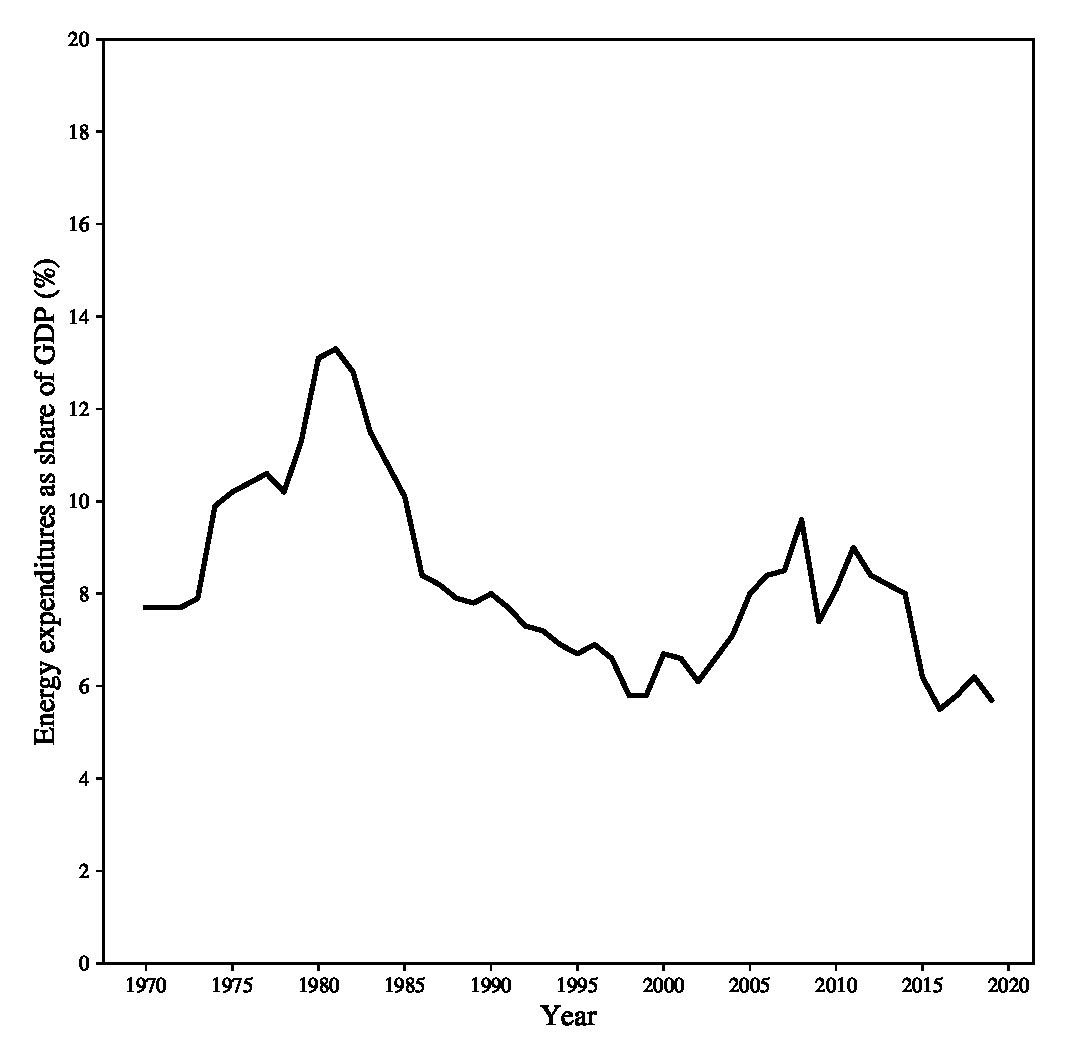
\includegraphics[height=3in]{../Figures/fig-ch10-fig1.eps}
\end{center}
\end{frame}

\begin{frame}{Energy intensity, $E_t/Y_t$}
\begin{center}
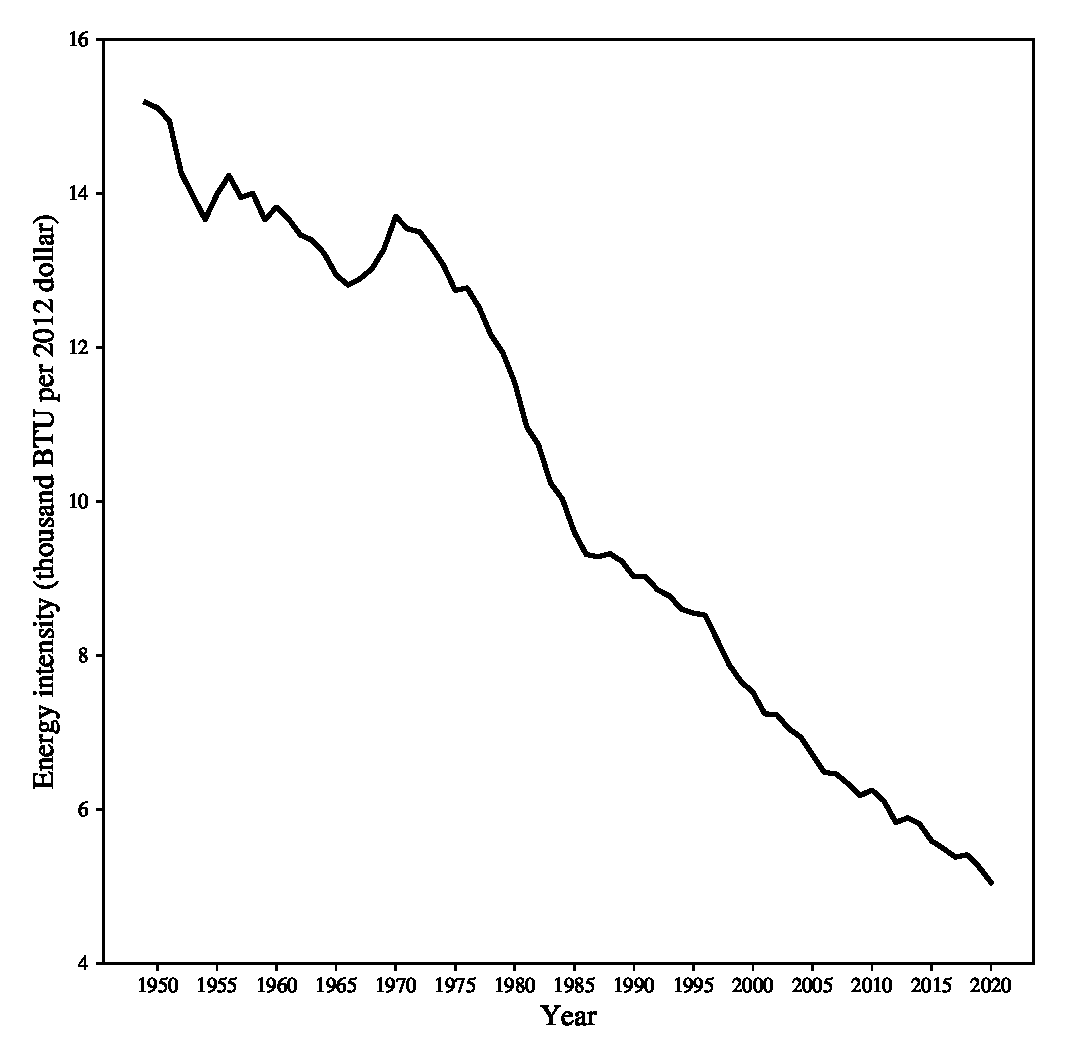
\includegraphics[height=3in]{../Figures/fig-ch10-fig2.eps}
\end{center}
\end{frame}

\begin{frame}{Implied price, $p_E$}
\begin{center}
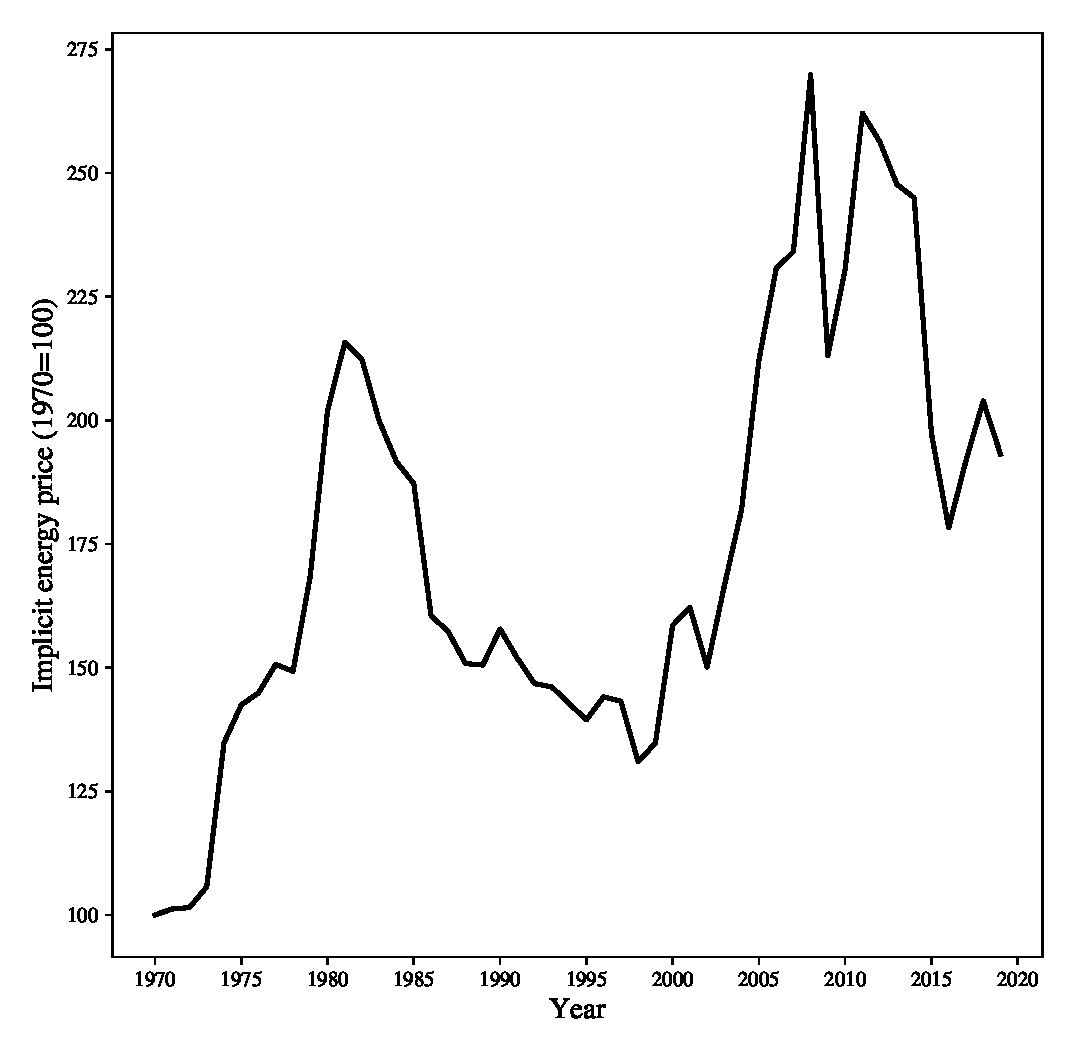
\includegraphics[height=3in]{../Figures/fig-ch10-fig3.eps}
\end{center}
\end{frame}

\begin{frame}{Total energy use}
\begin{center}
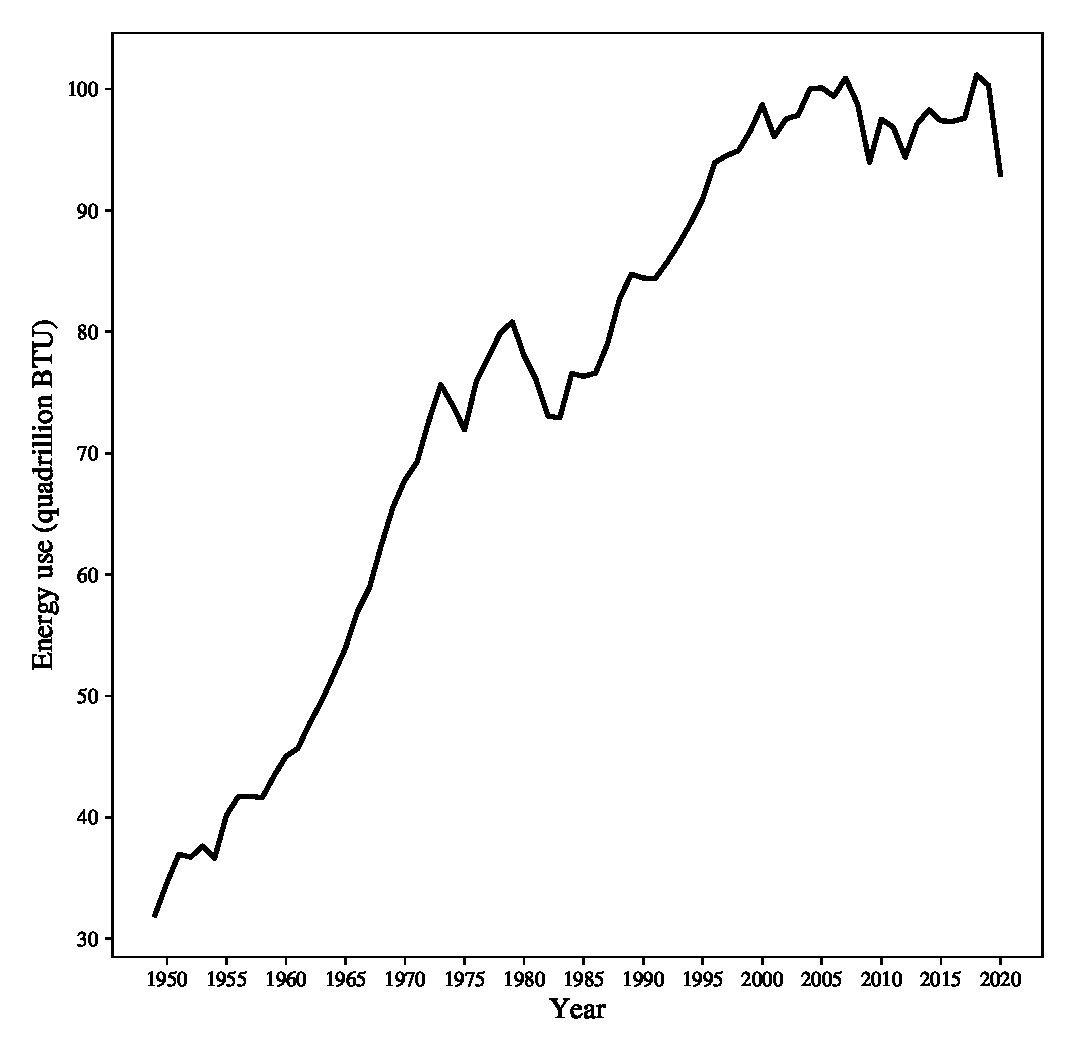
\includegraphics[height=3in]{../Figures/fig-ch10-fig4.eps}
\end{center}
\end{frame}

\begin{frame}{Declining share}
But is the energy share declining? An alternative production structure would give us
\begin{equation}
	Y_t = \left(K_t^{\rho} + (A_tE_t)^{\rho}\right)^{1/\rho}, \label{EQ_Y_CES}
\end{equation}
that ignores labor. 
\begin{itemize}
	\item $\rho$ determines how substitutable capital and energy are.
	\item If $0<\rho<1$ then they are easy to substitute
	\item If $\rho<0$ then they are complements (hard to substitute)
	\item $A$ is the productivity of energy specifically
\end{itemize}
\end{frame}

\begin{frame}{Energy Share}
With this model energy's share of GDP is
\begin{equation}
	\frac{p_{Et} E_t}{Y_t} = \left(\frac{A_tE_t}{Y_t}\right)^{\rho}. \nonumber
\end{equation}
\begin{itemize}
	\item We know $E/Y$ went down
	\item If $\rho > 0$ (substitutes) then this explains the declining share
	\item If $\rho < 0$ (complements) then share should go up, unless $A$ increased by a lot
	\item Seems like complements is more accurate (think a car and gas), so energy productivity $A$ must have gone up?
\end{itemize}
\end{frame}

\section{Growth and the environment}
\begin{frame}{The choice of $s_E$}
Like other rates, extraction is a choice. What might that decision look like?
\begin{equation}
	U_t = (c_t-\overline{c})^{1-\rho}R_t^{\rho} \label{EQ_U_cR}
\end{equation}
\begin{itemize}
	\item People care about consumption, $c$
	\item There is some minimum consumption, $\overline{c}$, that they need to have
	\item People care about the stock of resources, $R$
	\item That could be value of oil remaining in the ground
	\item Or that could be value of a forest or clean water
\end{itemize}
\end{frame}

\begin{frame}{Marginal utilies}
For consumption
\begin{equation}
	MU_c = \frac{(1-\rho)U_t}{c_t-\overline{c}} = (1-\rho)\frac{R_t^{\rho}}{(c_t-\overline{c})^{\rho}}. \label{EQ_MUc_R}
\end{equation}
and for resources
\begin{equation}
	MU_R = \frac{\rho U_t}{R_t} = \rho \frac{(c_t-\overline{c})^{1-\rho}}{R_t^{1-\rho}}. \label{EQ_MUR_R}
\end{equation}
In both cases, the MU goes down as you get more of the thing.
\end{frame}

\begin{frame}{Optimizing}
Set ratio of MU equal to ratio of prices
\begin{equation}
	\frac{MU_R}{MU_c} = \frac{P_{Rt}}{P_{ct}}
\end{equation}
as usual. But what are the prices? 
\end{frame}

\begin{frame}{Production and prices}
Let 
\begin{equation}
	y_t = E_t^{\beta} A_t^{1-\beta} L_t^{-\beta}, \label{EQ_y_R}
\end{equation}
be production per capita, and let $c_t = y_t$ (no capital). Also, the resource evolves
\begin{equation}
	dR = - E_t, \label{EQ_dotR_utility}
\end{equation}
So there is a trade-off in using $E_t$. It raises consumption but lowers the resource stock. 
\end{frame}

\begin{frame}{Production and prices}
\begin{equation}
	\frac{P_{Rt}}{P_{ct}} = \frac{\beta y_t/E_t}{1}.\nonumber
\end{equation}
\begin{itemize}
	\item The price of consumption is 1. It takes one unit of output to produce one unit of consumption.
	\item The price of the resource is $\beta y_t/E_t$. You have to sacrifice that amount of output (the MP of E) to keep one unit of $R$
\end{itemize}
\end{frame}

\begin{frame}{The optimal choice}
Solve for
\begin{equation}
	\frac{\rho (c_t-\overline{c})}{(1-\rho)R_t} = \beta \frac{y_t}{E_t}. \nonumber
\end{equation}
which is re-arranged into
\begin{equation}
	s_{Et} = \frac{E_t}{R_t} = \beta \frac{1-\rho}{\rho} \frac{y_t}{y_t-\overline{c}}. \label{EQ_sE_choice}
\end{equation}
and note it depends in two ways on the size of $y_t$.
\end{frame}

\begin{frame}{The environmental effects of growth}
With
\begin{equation}
	s_{Et} = \beta \frac{1-\rho}{\rho} \frac{y_t}{y_t-\overline{c}}. \label{EQ_sE_choice}
\end{equation}
\begin{itemize}
	\item If $y_t \rightarrow \overline{c}$ - poverty - then $s_{Et}$ is big 
	\item It makes sense to sacrifice $R$ to get more consumption
	\item But as $y_t$ gets very big via economic growth $s_{Et}$ goes down
	\item The additional consumption isn't worth very much compared to the loss of $R$
	\item It implies that environmental quality can improve with economic growth
	\item Think energy efficient cars/appliances, recycling, low-impact products, carbon offsets, etc..
\end{itemize}
\end{frame}

\begin{frame}{Energy use per capita}
\begin{center}
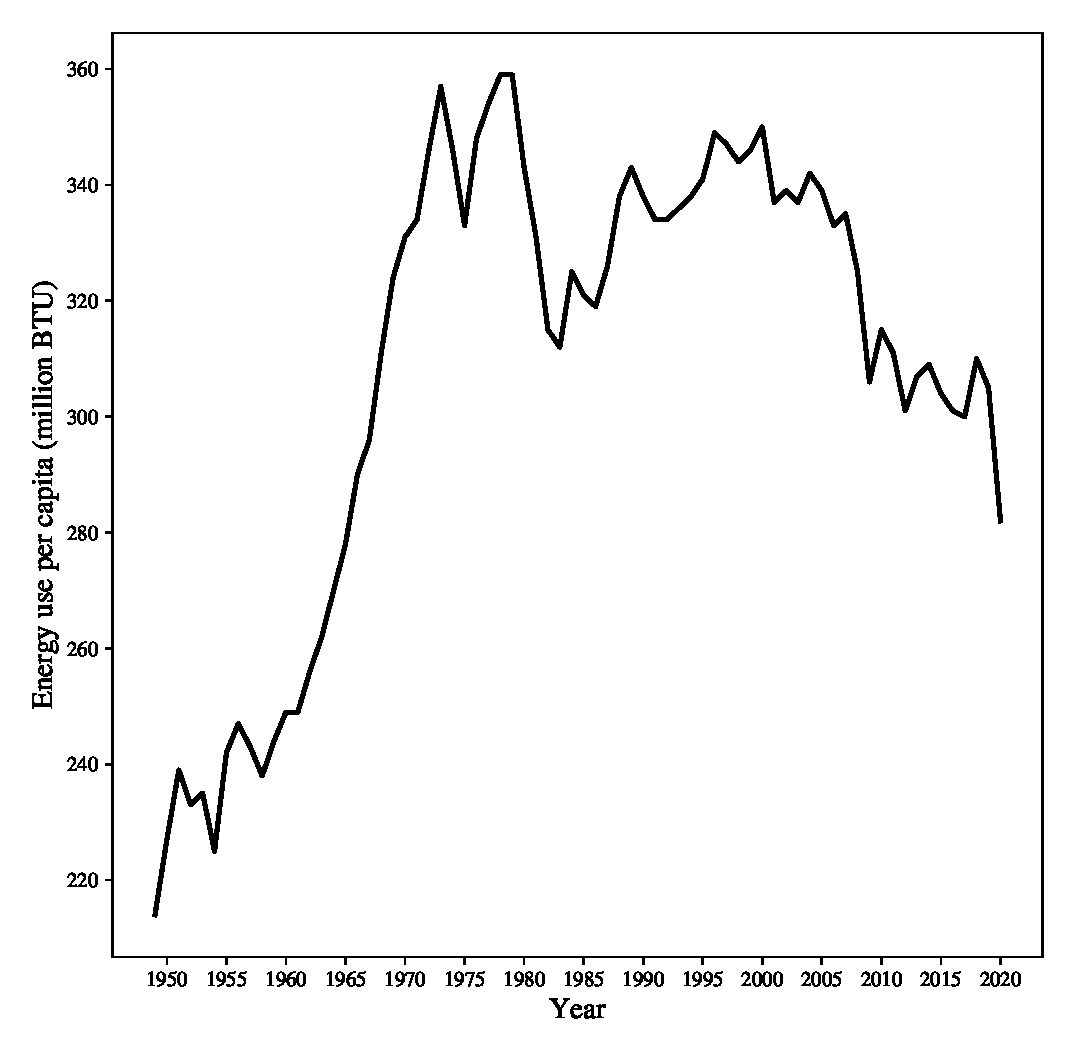
\includegraphics[height=3in]{../Figures/fig-ch10-fig5.eps}
\end{center}
\end{frame}

\begin{frame}{Total CO2 emissions}
\begin{center}
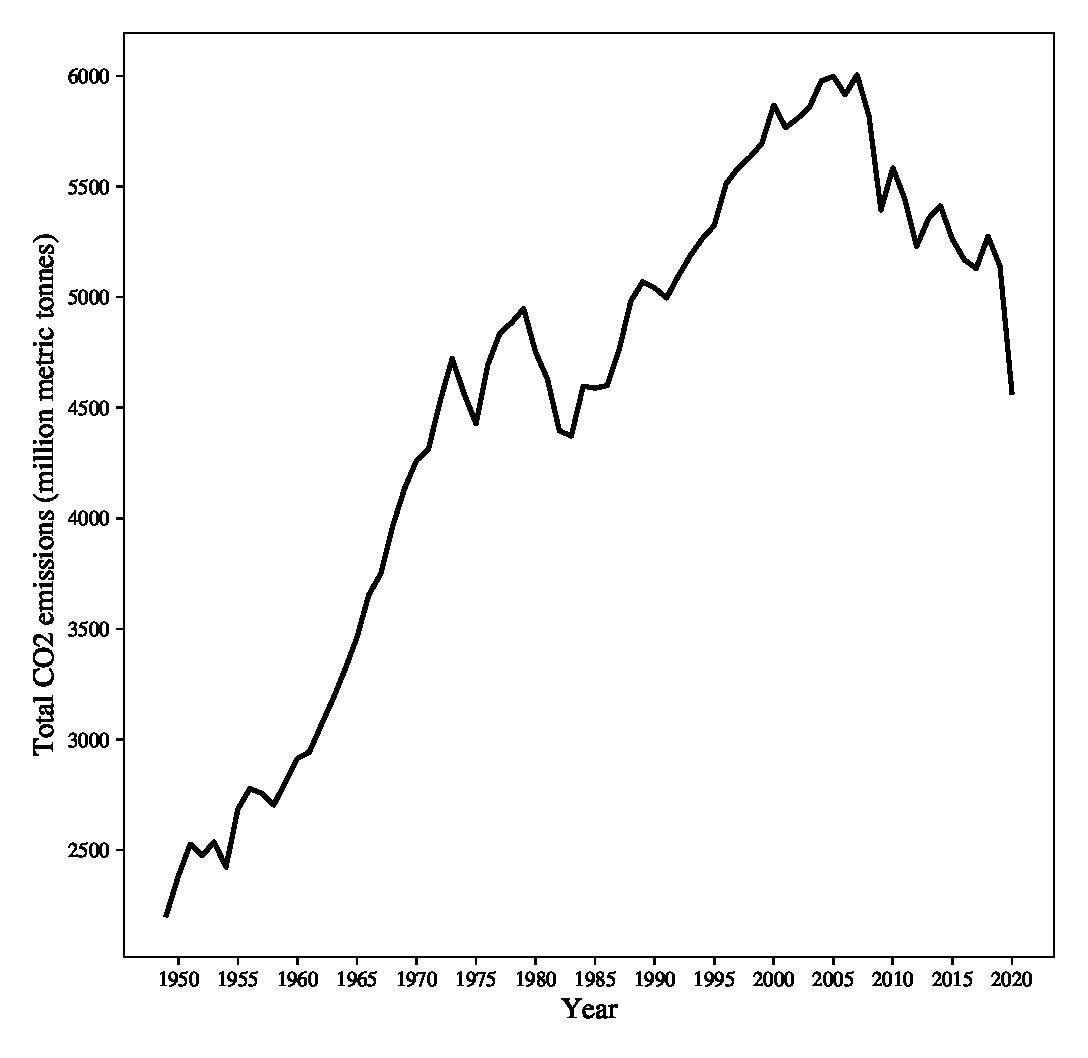
\includegraphics[height=3in]{../Figures/fig-ch10-fig6.eps}
\end{center}
\end{frame}

\begin{frame}{Renewable percent}
\begin{center}
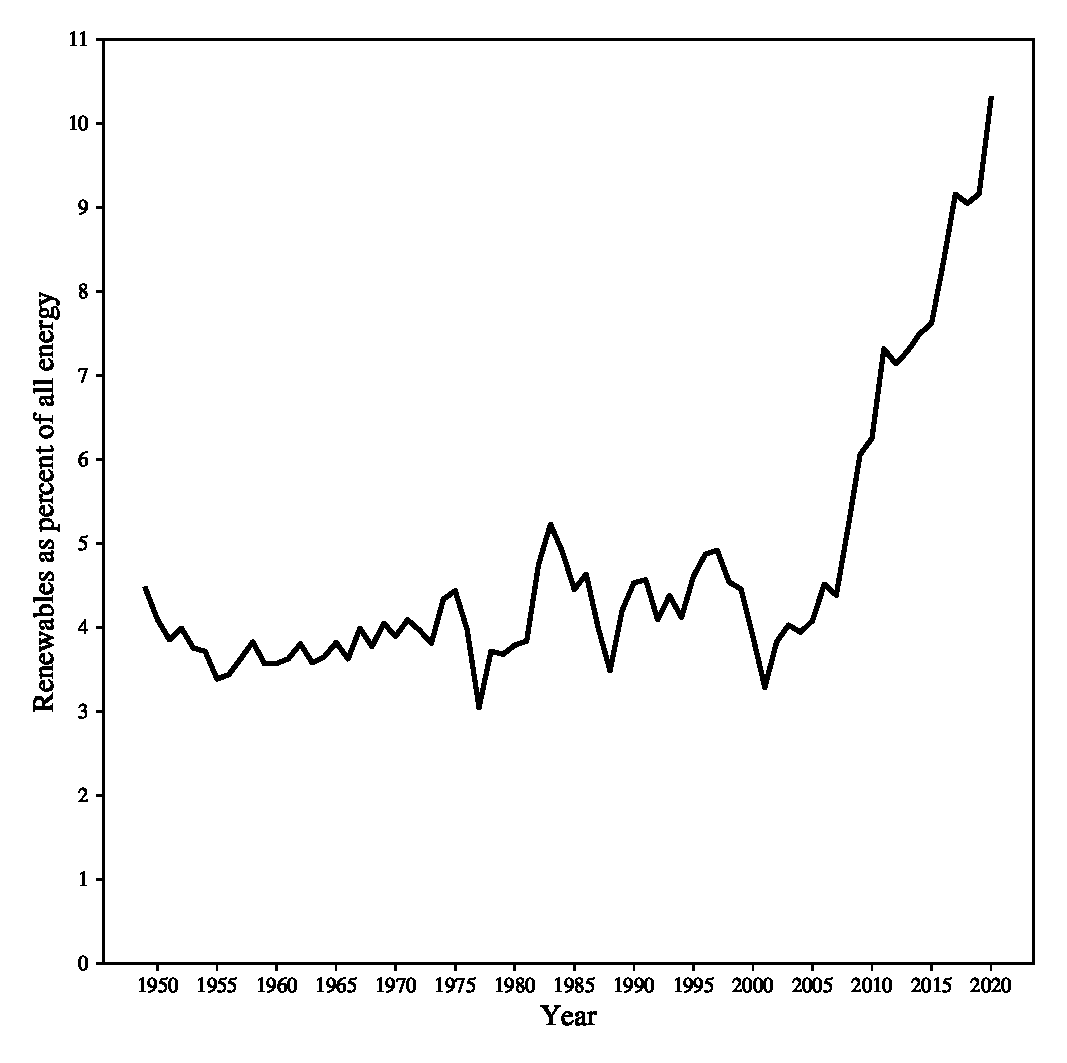
\includegraphics[height=3in]{../Figures/fig-ch10-fig7.eps}
\end{center}
\end{frame}

\begin{frame}{Air pollutants}
\begin{center}
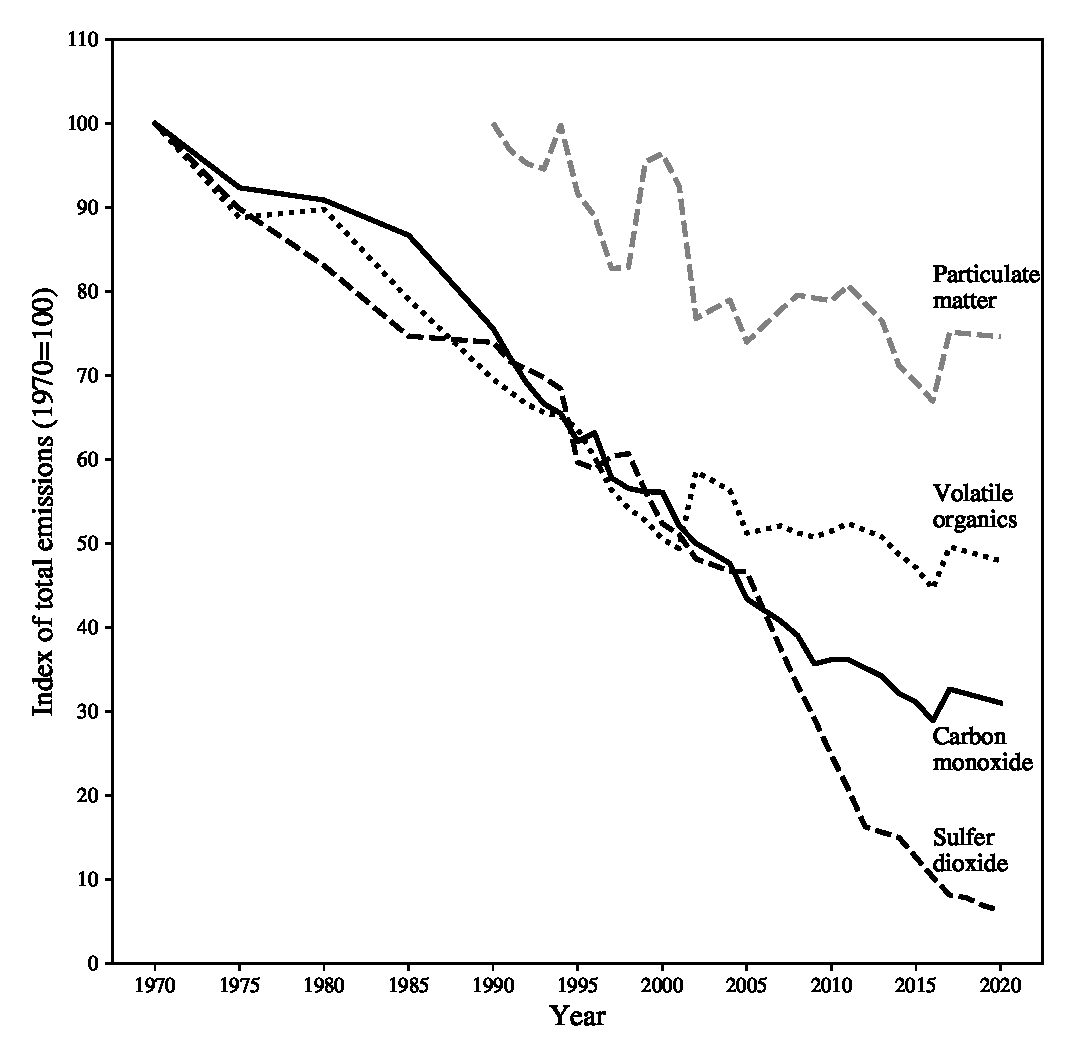
\includegraphics[height=3in]{../Figures/fig-ch10-fig8.eps}
\end{center}
\end{frame}

\end{document}